%%
%% This is file `sample-authordraft.tex',
%% generated with the docstrip utility.
%%
%% The original source files were:
%%
%% samples.dtx  (with options: `authordraft')
%% 
%% IMPORTANT NOTICE:
%% 
%% For the copyright see the source file.
%% 
%% Any modified versions of this file must be renamed
%% with new filenames distinct from sample-authordraft.tex.
%% 
%% For distribution of the original source see the terms
%% for copying and modification in the file samples.dtx.
%% 
%% This generated file may be distributed as long as the
%% original source files, as listed above, are part of the
%% same distribution. (The sources need not necessarily be
%% in the same archive or directory.)
%%
%% The first command in your LaTeX source must be the \documentclass command.
\documentclass[sigconf]{acmart}



%% NOTE that a single column version may be required for 
%% submission and peer review. This can be done by changing
%% the \doucmentclass[...]{acmart} in this template to 
%% \documentclass[manuscript,screen,review]{acmart}
%% 
%% To ensure 100% compatibility, please check the white list of
%% approved LaTeX packages to be used with the Master Article Template at
%% https://www.acm.org/publications/taps/whitelist-of-latex-packages 
%% before creating your document. The white list page provides 
%% information on how to submit additional LaTeX packages for 
%% review and adoption.
%% Fonts used in the template cannot be substituted; margin 
%% adjustments are not allowed.
%%
%% \BibTeX command to typeset BibTeX logo in the docs
\AtBeginDocument{%
  \providecommand\BibTeX{{%
    \normalfont B\kern-0.5em{\scshape i\kern-0.25em b}\kern-0.8em\TeX}}}

%% Rights management information.  This information is sent to you
%% when you complete the rights form.  These commands have SAMPLE
%% values in them; it is your responsibility as an author to replace
%% the commands and values with those provided to you when you
%% complete the rights form.
% \setcopyright{acmcopyright}
% \copyrightyear{2018}
% \acmYear{2018}
% \acmDOI{10.1145/1122445.1122456}

%% These commands are for a PROCEEDINGS abstract or paper.
% \acmConference[Woodstock '18]{Woodstock '18: ACM Symposium on Neural
%   Gaze Detection}{June 03--05, 2018}{Woodstock, NY}
% \acmBooktitle{Woodstock '18: ACM Symposium on Neural Gaze Detection,
%   June 03--05, 2018, Woodstock, NY}
% \acmPrice{15.00}
% \acmISBN{978-1-4503-XXXX-X/18/06}


%%
%% Submission ID.
%% Use this when submitting an article to a sponsored event. You'll
%% receive a unique submission ID from the organizers
%% of the event, and this ID should be used as the parameter to this command.
%%\acmSubmissionID{123-A56-BU3}

%%
%% The majority of ACM publications use numbered citations and
%% references.  The command \citestyle{authoryear} switches to the
%% "author year" style.
%%
%% If you are preparing content for an event
%% sponsored by ACM SIGGRAPH, you must use the "author year" style of
%% citations and references.
%% Uncommenting
%% the next command will enable that style.
%%\citestyle{acmauthoryear}
\settopmatter{printacmref=false} % Removes citation information below abstract
\renewcommand\footnotetextcopyrightpermission[1]{} % removes footnote with conference information in first column
\pagestyle{plain} % removes running headers

%% end of the preamble, start of the body of the document source.
\begin{document}

%%
%% The "title" command has an optional parameter,
%% allowing the author to define a "short title" to be used in page headers.
\title{High Resolution Topic Modeling}

%%
%% The "author" command and its associated commands are used to define
%% the authors and their affiliations.
%% Of note is the shared affiliation of the first two authors, and the
%% "authornote" and "authornotemark" commands
%% used to denote shared contribution to the research.
\author{Viren Bajaj}
% \authornote{Both authors contributed equally to this research.}
\email{vb2519@columbia.edu}
% \orcid{1234-5678-9012}
\affiliation{%
  \institution{Columbia University}
%   \streetaddress{P.O. Box 1212}
  \city{New York}
  \state{NY}
  \country{USA}
%   \postcode{43017-6221}
}
\author{Mark Aksen}
% \authornote{Both authors contributed equally to this research.}
\email{mja2213@columbia.edu}
% \orcid{1234-5678-9012}
\affiliation{%
  \institution{Columbia University}
%   \streetaddress{P.O. Box 1212}
  \city{New York}
  \state{NY}
  \country{USA}
%   \postcode{43017-6221}
}
%%
%% By default, the full list of authors will be used in the page
%% headers. Often, this list is too long, and will overlap
%% other information printed in the page headers. This command allows
%% the author to define a more concise list
%% of authors' names for this purpose.
% \renewcommand{\shortauthors}{Viren Bajaj}

%%
%% The abstract is a short summary of the work to be presented in the
%% article.
\begin{abstract}
Typical paper recommendation systems offer results on a document level.Yet in practice, different citations are sought after in different sections of the paper. Furthermore, often the most appropriate citations can be from different academic communities. We present a versatile citation recommendation system that can provide accurate inference for smaller texts, recommendations across domains, and usage of known citation networks. First, we evaluate the quality of inference provided by LDA, LDA with word embeddings, and LDA with word embeddings and citation network on the sub-document (section and paragraph) levels using the SemanticScholar dataset. We found that LDA with word embeddings and citation networks performs better on key metrics of mean precision, recall, F-measure, and reciprocal rank. 
Using our findings, we develop an LDA model augmented with citation networks in a new way.
We show that it outperforms other models on the above metrics, especially improving cross-domain recommendations. 

\end{abstract}

\settopmatter{printacmref=false} %% to remove ACM reference format box


%%
%% Keywords. The author(s) should pick words that accurately describe
%% the work being presented. Separate the keywords with commas.
\keywords{Topic Modelling, LDA}

%% A "teaser" image appears between the author and affiliation
%% information and the body of the document, and typically spans the
%% page.
% \begin{teaserfigure}
%   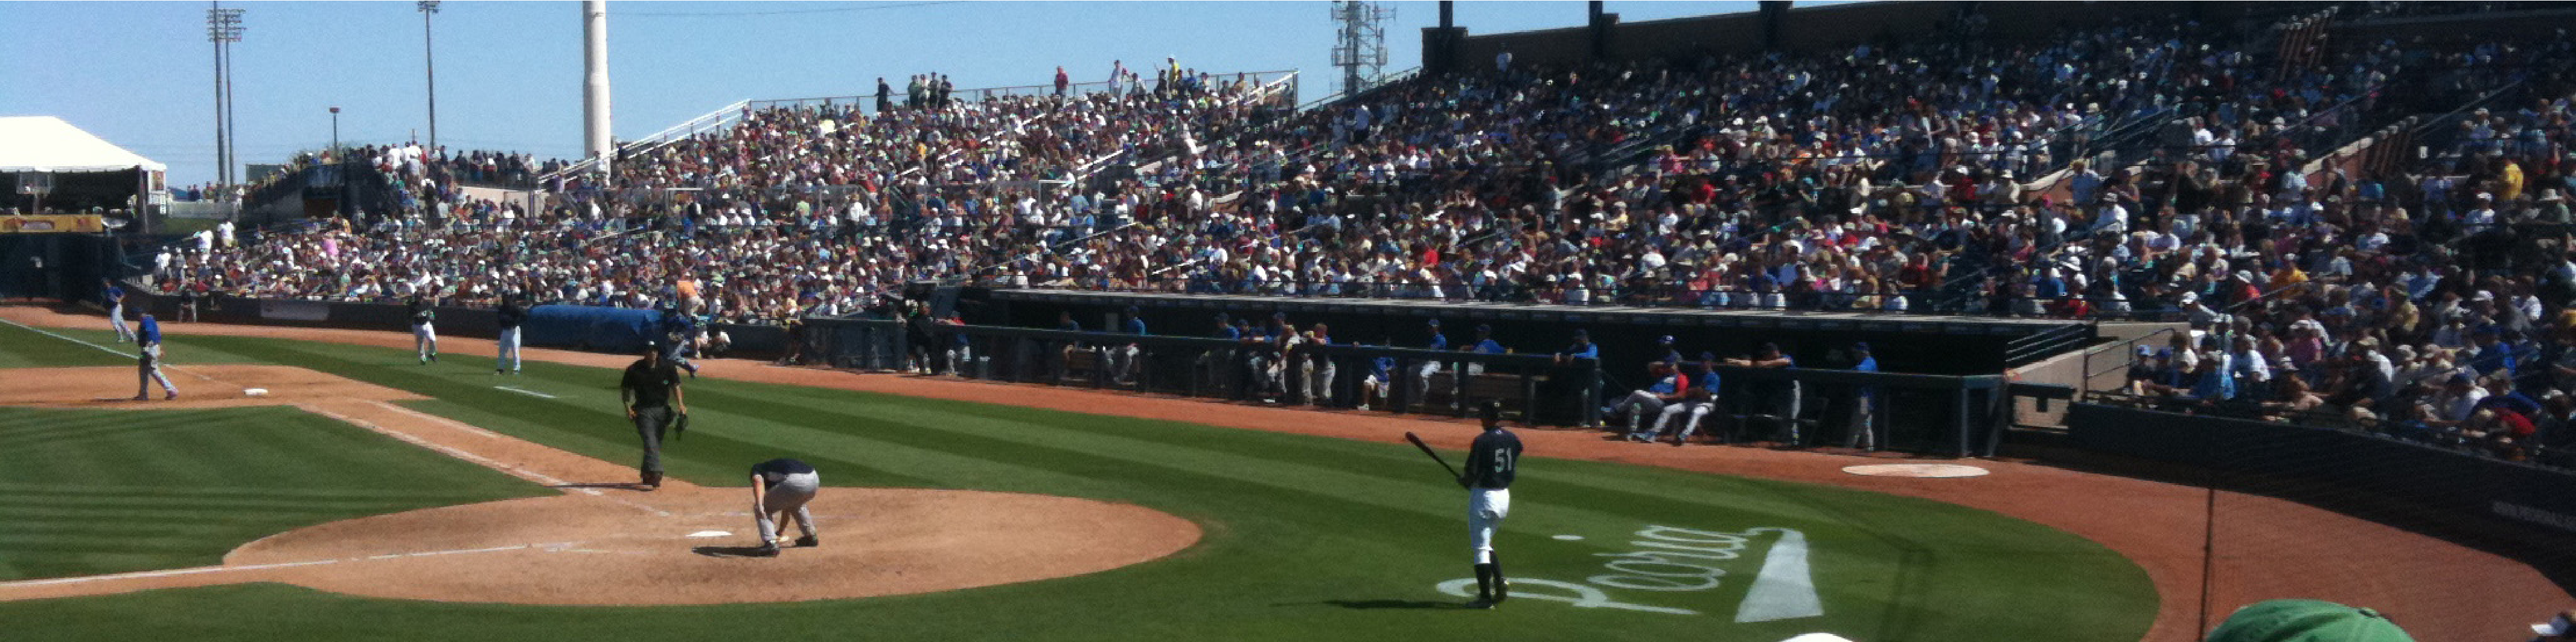
\includegraphics[width=\textwidth]{sampleteaser}
%   \caption{Seattle Mariners at Spring Training, 2010.}
%   \Description{Enjoying the baseball game from the third-base
%   seats. Ichiro Suzuki preparing to bat.}
%   \label{fig:teaser}
% \end{teaserfigure}

%%
%% This command processes the author and affiliation and title
%% information and builds the first part of the formatted document.
\maketitle
\section{Introduction}
Latent Dirichlet Allocation is an effective way to understand the topics addressed in a document on a semantic level. Current implementations of topic models on different data sets focus on assigning topics on a document level, or the 'global' level. In reality, however, the topics addressed in a document vary by paragraph or section or the 'local' level. For example, most scientific papers contain an section to introduce the global topic , a background section that discusses different topics in subsections, a section to discuss the main problem and proposed solutions, and finally a conclusion. Less formal documents often also contain an implicit structure in which different topics are discussed at different points in the document. Thus a 'high resolution' topic model that can uncover topics on a finer scale than the entire document is desirable.

An important implication of being able to detect topics at the local level is that it engenders a completely new way to conduct self-directed learning. Today, the way to learn a new topic depends on the difficulty of the topic: simple facts and how-to's are query-able using short, well defined strings through an internet search engine; more difficult topics are explained through articles, tutorials, or books found on the internet; and exploring complete subjects requires enrolling in a course provided by an educational institution - either online or in-person. The reason learning complete subjects on your own is not advised is obvious - one doesn't know where to start studying and how to go about exploring the subject matter in an reasonably efficient way. We claim that a high resolution topic model empowers a learner to explore arbitrary subject areas in a more efficient way than haphazard internet searches and thereby help everyone learn new and complex material faster. 

High resolution topic modeling provides an automatic way to extract the topics in paragraph (or other document quanta), which gives a learner two ways to explore content related to the given paragraph. The first and more obvious way that a learner can explore the topics implicit in a given paragraph is by finding other document quanta that resemble its topic make up the most. This is essentially asking for recommendations of similar text. The second and more interesting way is by being able to explore each of the topic-spaces on their own. A topic-space is the list of document quanta that mention that topic. This means being able to find document quanta that have the highest proportion of a given topic. Further ranking of document quanta in topic-space can be achieved with algorithms that use citation networks such as PageRank [], which would give learners access to the most relevant document quanta for a topic - a topic that they didn't have to explicitly search for.  A search system built using a high resolution topic model can thus alleviate the problem of unknown unknowns (we can't search for things we don't know we need to search for) during the learning process. Therefore, such a system can guide a learner in uncovering information that not only implicitly resembles their document quanta, i.e., their search query, but also the most important information pertaining to that topic, thereby creating a guided search process that mimics an educational course.  


\section{Background}
A little history of Topic modeling ...


\subsection{Latent Dirichlet Allocation}

\href{http://www.cse.cuhk.edu.hk/irwin.king/_media/presentations/latent_dirichlet_allocation.pdf}{BLEI LDA 1}
\subsubsection{Word Embeddings}
rumelhart 1973 word embeddings
blei maya rudolph exponential family embeddings
estia bengio neural language modelling
Check this out for word embeddings:\\
\href{https://towardsdatascience.com/lda2vec-word-embeddings-in-topic-models-4ee3fc4b2843}{1}
\href{https://multithreaded.stitchfix.com/blog/2016/05/27/lda2vec/#topic=3&lambda=1&term=}{2}
\href{https://www.aclweb.org/anthology/P15-1077.pdf}{3}
\href{https://arxiv.org/pdf/1604.00126.pdf }{4}

\subsubsection{Citation Networks}

\subsubsection{Collaborative Filtering}

\subsubsection{Any work on high resolution??}

\subsubsection{Cross-domain Accuracy}

\section{High Resolution Experiments}

\subsection{Data}

\subsection{Section-scale}

\subsection{Paragraph-scale}

\section{Conclusion}
%%
%% The next two lines define the bibliography style to be used, and
%% the bibliography file.
\bibliographystyle{ACM-Reference-Format}
\bibliography{sample-base}

%%
%% If your work has an appendix, this is the place to put it.
% \appendix

\end{document}
\endinput
%%
%% End of file `sample-authordraft.tex'.
